\section{ArduPilot SITL setup}
First thing we want to do is setting up Ardupilot \gls{sitl}.
We do that by following the official guide to make it work under the \gls{wsl} system on a Windows 11 \gls{pc}.
This will also create a special Python environment to better manage packages and modules needed to run Ardupilot.

After setting all up we start it up by using a special command:
\begin{minted}[breaklines]{bash}
    python3 /home/darckat038/uni/cps/ardupilot/Tools/autotest/sim_vehicle.py -v ArduCopter --console --map --mavproxy-args="--load-module=batteryreset --out=127.0.0.1:14550 --out=127.0.0.1:14549 --out=127.0.0.1:14548 --out=127.0.0.1:14547 --out=127.0.0.1:14546 --out=127.0.0.1:14545 --cmd=\"param set RTL_ALT_FINAL_M 15\""
\end{minted}

With this command we are able to:
\begin{itemize}
    \item use the ArduCopter as represented vehicle;
    \item show the console and the map to better visualize the drone movement and flight status;
    \item set alternative output ports to communicate with MAVProxy using multiple programs;
    \item set a final altitude for the \gls{rtl} mode.
          \begin{figure}[H]
              \centering
              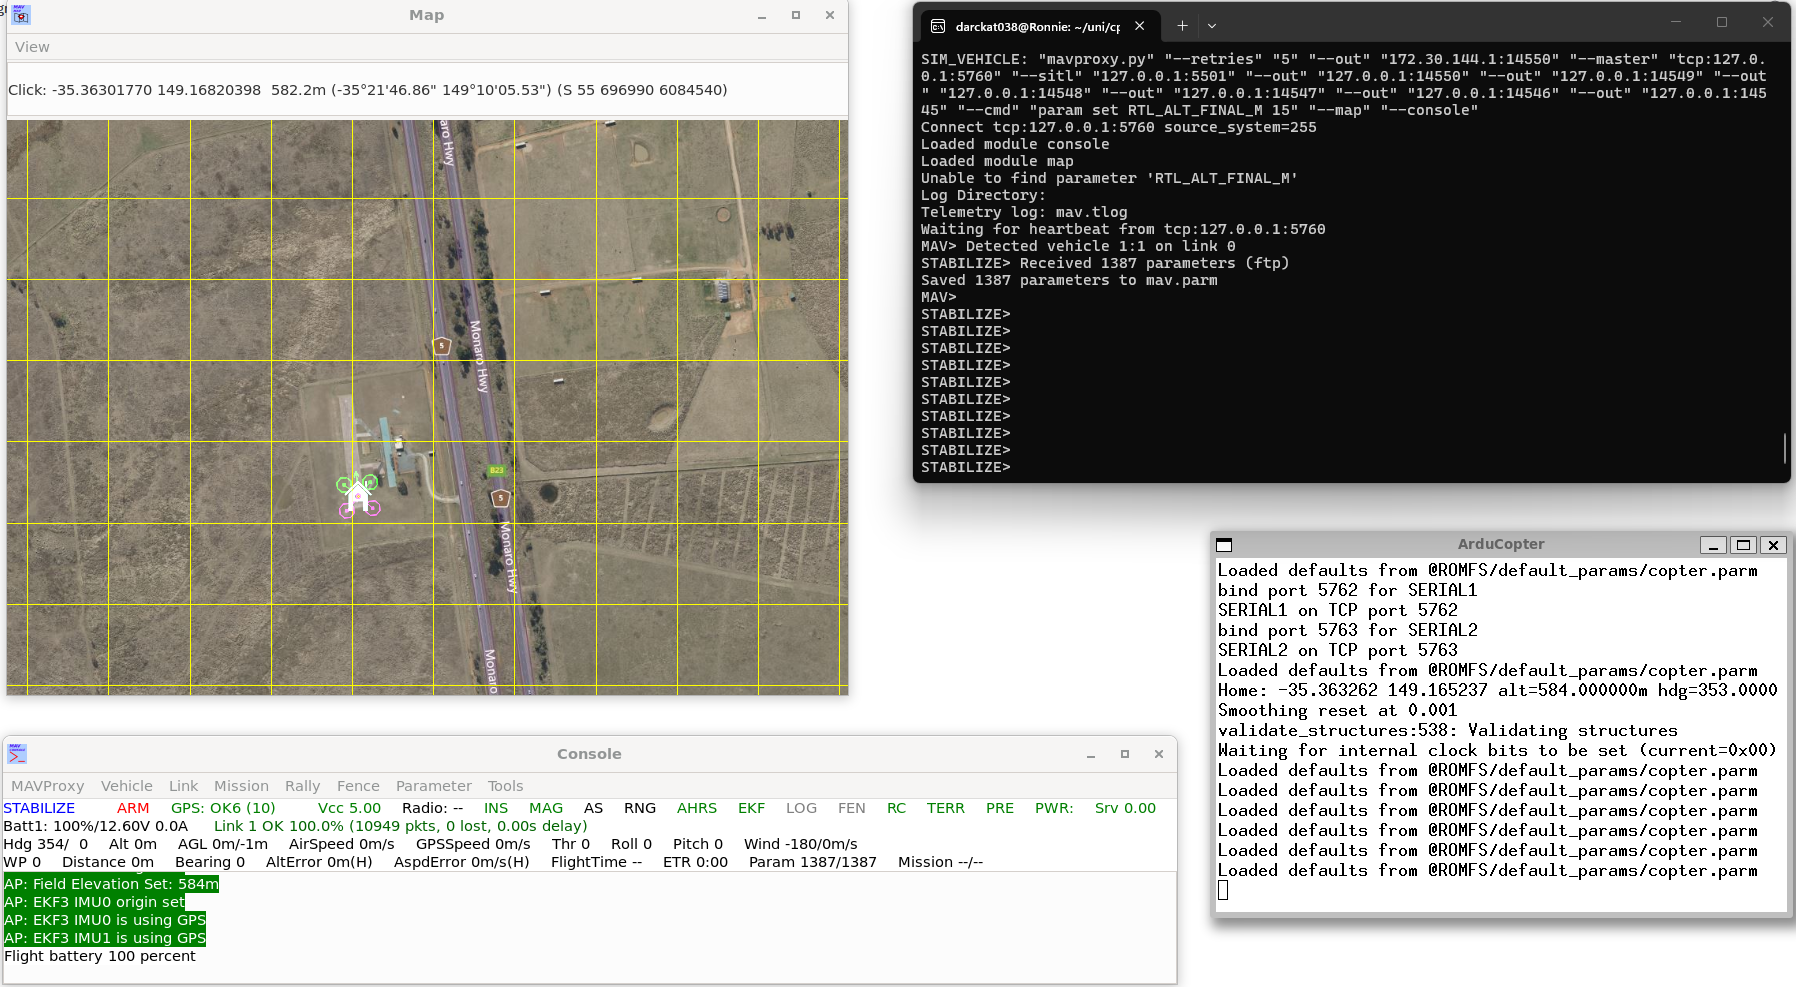
\includegraphics[width=.8\linewidth]
              {Data/Images/ardupilot_setup.png}
              \caption{Final Ardupilot \gls{sitl} workplace.}
              \label{fig:ardupilot_workplace}
          \end{figure}
\end{itemize}

\section{Python helper}
To better achieve what we need we decided to create multiple Python classes, thus dividing responsibilities among multiple parts of the program.

\subsection{GPSReader}
The first and most important is the \texttt{GPSReader} class.
This particularly useful Python class enabled us to continuously request the \gls{gps} position of the drone from the MAVProxy software by using a specifically exposed \gls{api}, accessible through the ports we requested in the launch command.
Latitude, Longitude and Altitude were the main requested parameters.

\subsection{FlightMonitor}
Then comes \texttt{FlightMonitor}, which helped mainly to acquire information about the ongoing mission like the number of waypoints, the index of the landing waypoint and so on.
Were also included function to gather information about events and status changes which helped us better understand the thresholds and limits supported by the flight controller.

\subsection{GlitchController}
The \texttt{GlitchController} class, as the name says, had the obvious goal of setting and getting the desired glitch parameters through an \gls{api} endpoint.

\subsection{FlightLogger}
To \texttt{FlightLogger} class has then been given the task of logging every step of the \gls{gps} of the drone, along with the currently set glitch and any events that may occur during the spoofing period.

\subsection{Other utils}
\subsubsection{Distance}
A \texttt{distance} method has been written to compute the distance between two coordinates and help with the progressive/adaptive glitch computations and development.